\documentclass[amsmath,amssymb,notitlepage,11pt]{revtex4}
%\documentclass[12pt]{article}
\usepackage{graphicx}
\usepackage{bm}% bold math
\usepackage{multirow}
\usepackage{booktabs}
\usepackage{verbatim}
\usepackage{hyperref}
\usepackage{enumitem}
\hypersetup{pdftex,colorlinks=true,allcolors=blue}
\usepackage{hypcap}
\usepackage[small,compact]{titlesec}
\setlist[enumerate]{itemsep=0mm}

\begin{document}
\title{CLAS12 Slow Controls Operations Manual - v1.2}
\date{\today}
\begin{abstract}
\end{abstract}

\maketitle
%\tableofcontents
%\newpage

\section{Overview}
The operator interface for the Hall B controls systems is based on Control System Studio (also called CS-Studio or CSS) and allows access to all the necessary EPICS tools from a single application.  This system is accessible locally by user \texttt{clasrun} from all \texttt{clonpc\#\#} desktop computers in the Hall B Counting Room for shift workers.  There are also \texttt{clonsl\#} servers for remote use with access to the same software.  All controls computers are behind JLab's \texttt{hallgw} gateway and require 2-factor authentication for remote access.

To start the control system with only the main menu as shown in the left panel of Figure~\ref{fig:mainmenu}, in a terminal run: \begin{center}\texttt{clascss}\end{center}
To start the control system with the full alarm handler as shown in the right panel of Figure~\ref{fig:mainmenu}, in a terminal run:
\begin{center}\texttt{clascss-alarm}\end{center}

\begin{figure}[htpb]\centering
    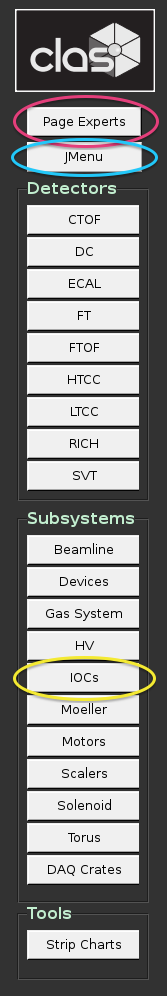
\includegraphics[width=0.08\textwidth]{pics/mainmenu}\hspace{0.5cm}
  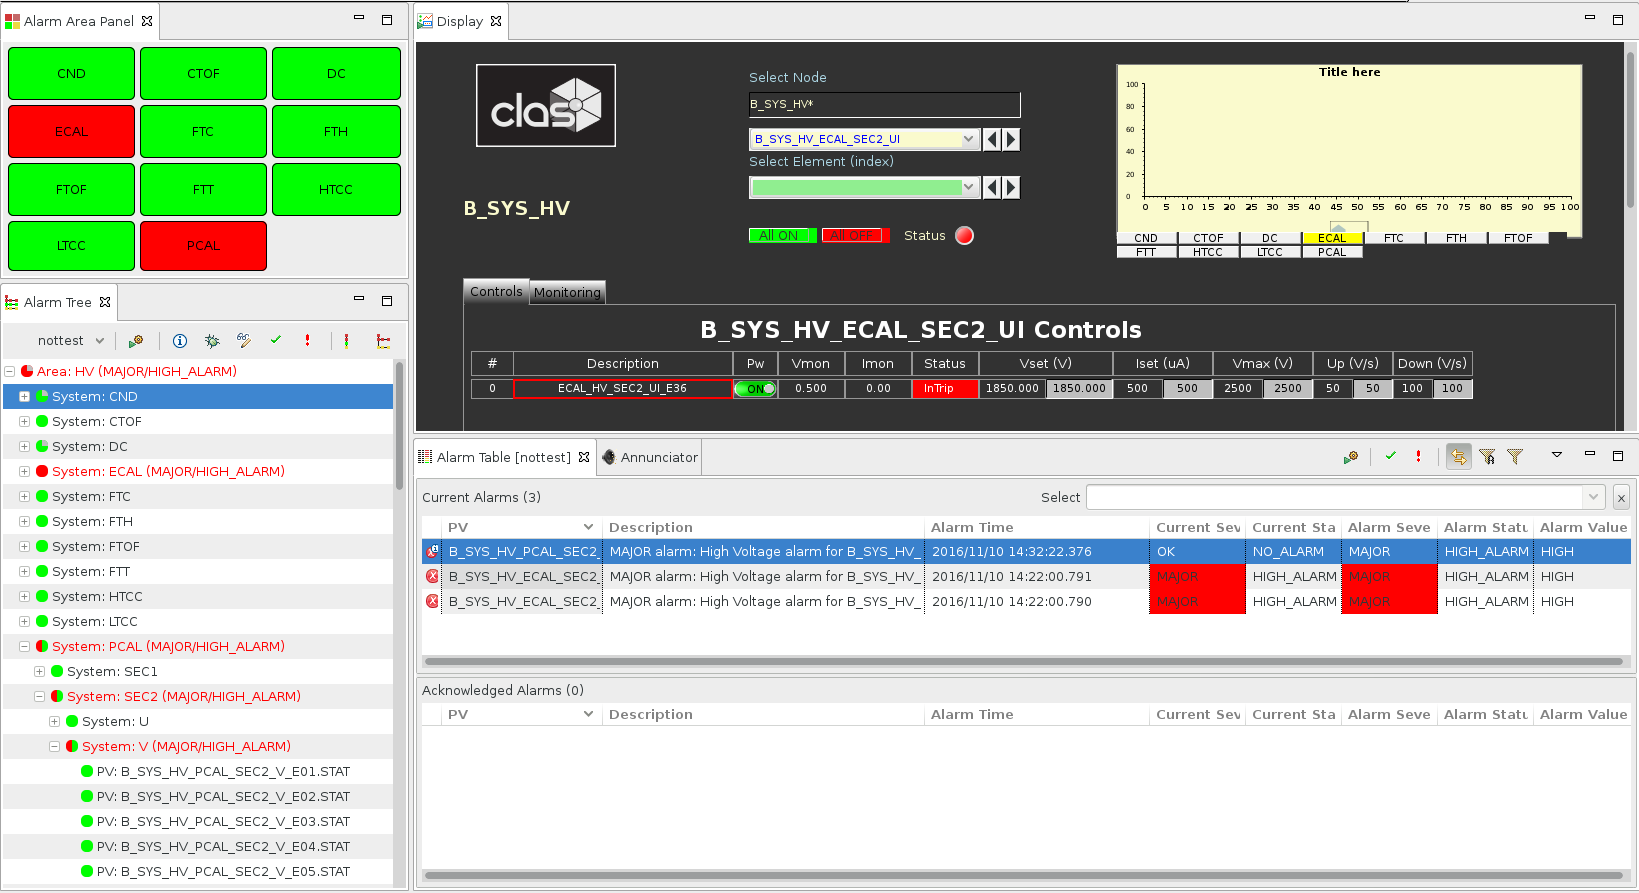
\includegraphics[width=0.88\textwidth]{pics/clas12alarm}
  \caption{On the left is the main CLAS12 controls menu showing locations of buttons used for the accelerator's JMenu screens (blue), paging Hall-B experts (pink), and restarting IOCs (yellow).  On the right is the alarm controls screen.\label{fig:mainmenu}}
\end{figure}

The main menu is organized in a hierarchy of subsystems and components.  The top portion of the menu is for specific detectors, while the bottom portion is for more general subsystems.  The alarm screen is organized into different regions described in the following sections.

\section{Alarms}

The user frontend of the alarm handling system runs in CS-Studio and includes visual and audible alarms.  The default alarm view when running \texttt{clascss-alarm} is shown in the right panel of Figure~\ref{fig:mainmenu}.  On the left are the {\em Area Panel}, an overview of the systems' alarm statuses, and the {\em Alarm Tree}, a hierarchical view of all alarm settings.  The right side contains the {\em Alarm Table} (see also Figure~\ref{fig:alarmtree}), a list of active alarms that should be addressed and a separate list of already acknowledged alarms.  

\begin{figure}[htbp]\centering
  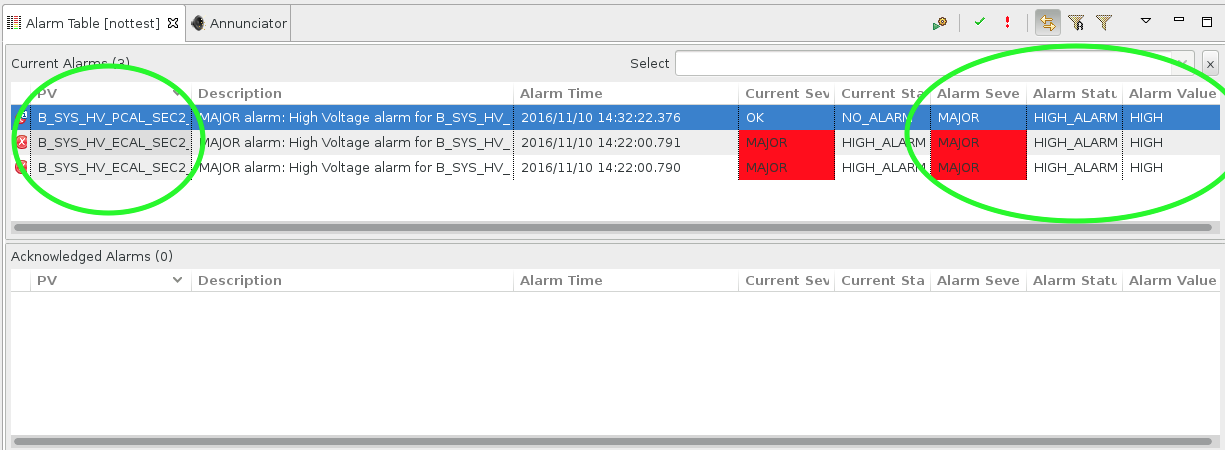
\includegraphics[width=0.99\textwidth]{pics/alarmtree}
  \caption{The {\em Alarm Tree} portion of the alarm screen, showing an example of three outstanding alarms that need to be addressed.  The first is no longer in an alarm state (denoted by the {\em OK} in the {\em Current Severity} column), and none of the three have been acknowledged (or else they would have appeared instead in the lower {\em Acknowledged Alarms} section).\label{fig:alarmtree}}
\end{figure}

By right-clicking on an alarm in the {\em Alarm Table}, a dropdown menu of actions is accessible (see Figure~\ref{fig:alarmguide}).  This dropdown list contains access to a {\em Guidance} screen with instructions that should be read and followed on how to deal with the specific alarm.  The next step is to acknowledge the alarm using the {\em Acknowledge} option in the dropdown menu, which will silence the alarm and move it to the {\em Acknowledged Alarms} section until it is no longer in an alarm state.  For many alarms there is also an option in the dropdown menu starting with {\em Open} that will open a screen necessary to address the specific alarm using the information from the {\em Guidance} screen.

\begin{figure}[htbp]\centering
  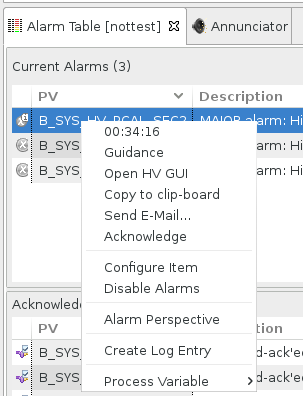
\includegraphics[width=0.3\textwidth]{pics/alarmguide}
  \caption{An example dropdown menu accessible by right-clicking on an alarm in the {\em Alarm Table}.  Important visible actions include a {\em Guidance} button, an {\em Open} screen action, and the {\em Acknowledge} action.\label{fig:alarmguide}}
\end{figure}


\section{IOCs}
EPICS input-output controllers (IOCs) are the backend responsible for the actual communication with the hardware devices in the hall.  Figure~\ref{fig:iocmenu} illustrates access to the IOC controls screens from the main CLAS12 menu, as well as the overview IOC heartbeat screen.  The heartbeats should be flashing at 1 Hz for all IOCs, or else the IOC may be in need of reboot.  By clicking on the IOC in the heartbeat screen (or the IOC health group in the main menu), controls to monitor and reboot the IOCs can be accessed, and an example is shown in Figure~\ref{fig:iochealth}.  Systems are in place to automatically start all necessary IOCs if for any reason they are not running (e.g. recovery from a power outage), however occaisonally a manual reboot is required.

\begin{figure}[htbp]\centering
  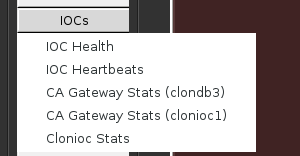
\includegraphics[width=0.25\textwidth]{pics/iocmenu}
  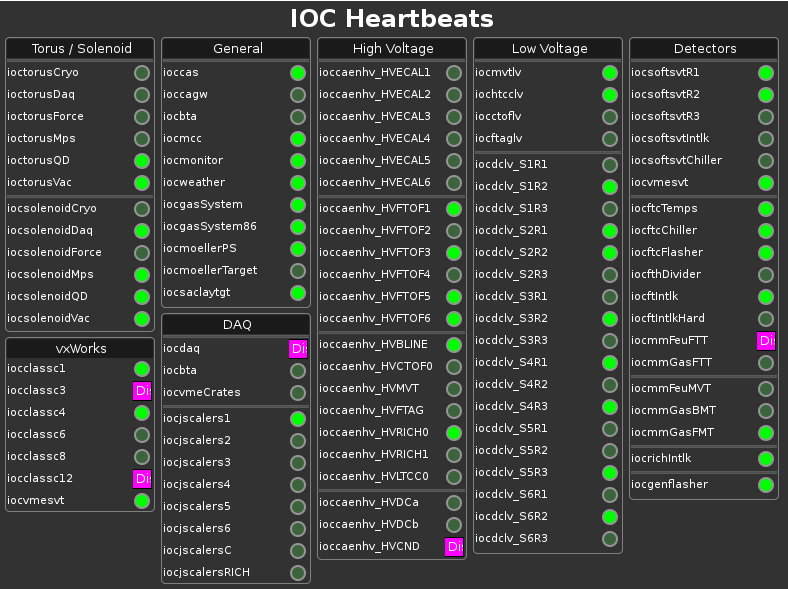
\includegraphics[width=0.45\textwidth]{pics/iocbeats}
  \caption{Dropdown menu (left) from the {\em IOCs} button in the main CLAS12 controls menu showing links to health screens for subsets of IOC groups, and the IOC heartbeat overview screen (right).\label{fig:iocmenu}}
\end{figure}

\begin{figure}[htbp]\centering
  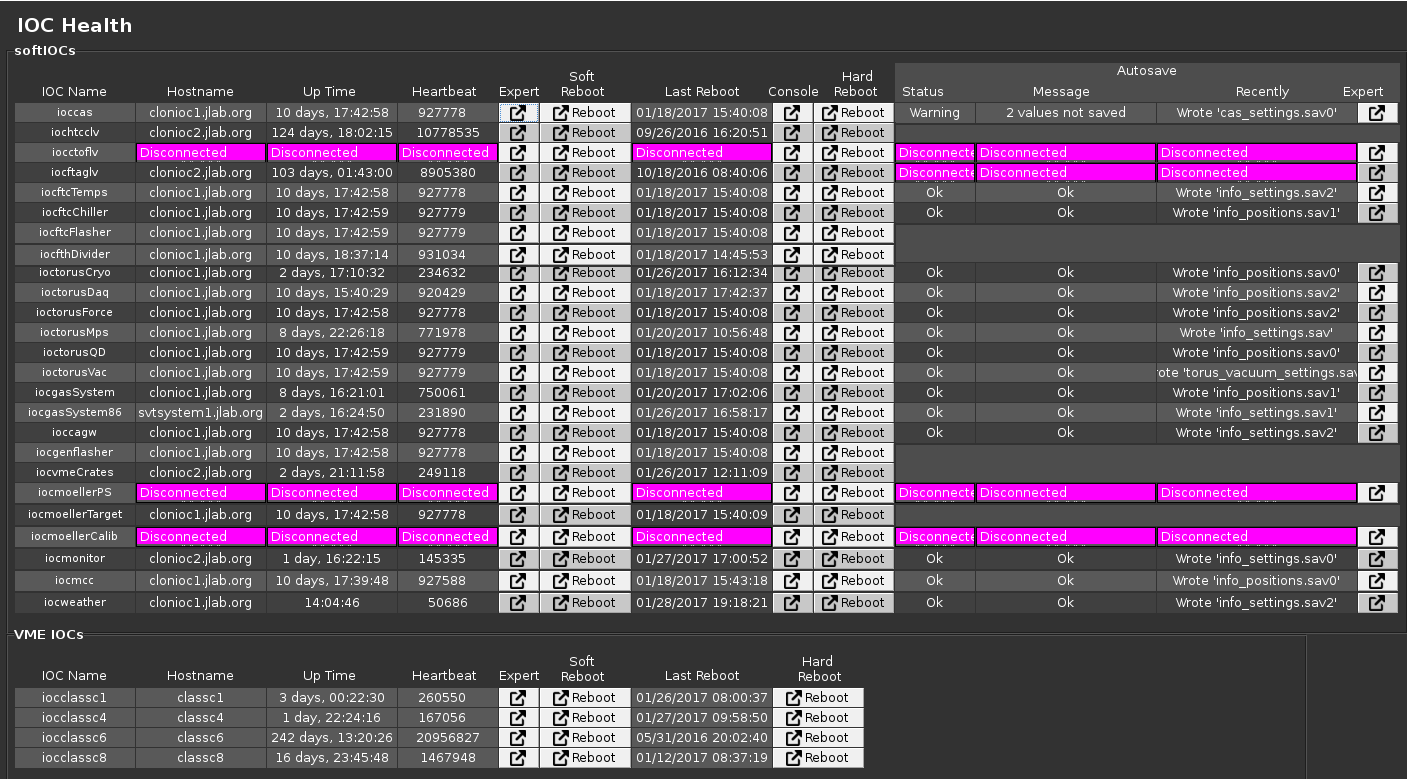
\includegraphics[width=\textwidth]{pics/iochealth}
  \caption{The primary IOC health screen showing uptime, heartbeats, and autosave status for each IOC, and buttons to restart them.  Pink rows designate IOCs that are not currently running in this screenshot, but under normal operations all rows should have normal readings.  \label{fig:iochealth}}
\end{figure}

\clearpage

\section{High Voltage}
The largest controls system in Hall B in terms of number of channels is high voltage (HV), with 23 CAEN crates including SY527, SY1527, and SY4527 mainframes.  An overview screen of the status of all HV in Hall B is accessible from the HV button in the main CLAS12 menu as shown in Figure~\ref{fig:hv}.  Clicking on a detector in this overview screen will bring up the HV controls for that detector (also accessible under each detector's button in the main menu).

\begin{figure}[htbp]\centering
  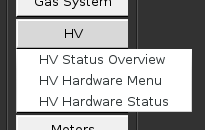
\includegraphics[width=0.3\textwidth]{pics/hvmenu}
  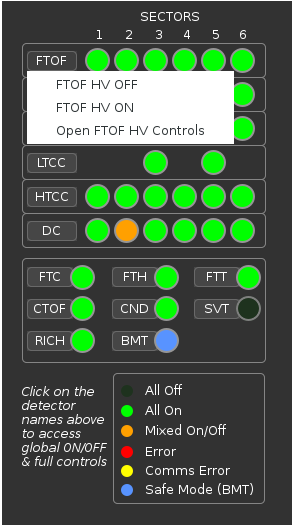
\includegraphics[width=0.2\textwidth]{pics/hvstat}
  \caption{Access to the HV overview screen from the main menu (left).  Clicking on a detector's name in the overview screen (right) will open its HV controls screen.\label{fig:hv}}
\end{figure}


\section{Strip Charts}
There are two applications available for plotting time histories of slow controls variables:  StripTool and MyaViewer.  Both are available from the {\em Strip Charts} button at the bottom of the main CLAS12 controls menu as shown in Figure~\ref{fig:strips}.

The suggested tool for online operations in Hall B is StripTool, which has no access to archived data but is very robust and stable.  MyaViewer is ideal for expert studies and can access the Mya archive used to store previous years of Hall B controls data.  In either case, configuration files are loadable from their user interfaces to view a predetermined set of variables, or else you can choose any process variable to plot.

\begin{figure}[htbp]\centering
    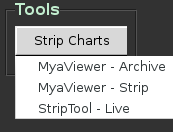
\includegraphics[width=0.2\textwidth]{pics/strips}
    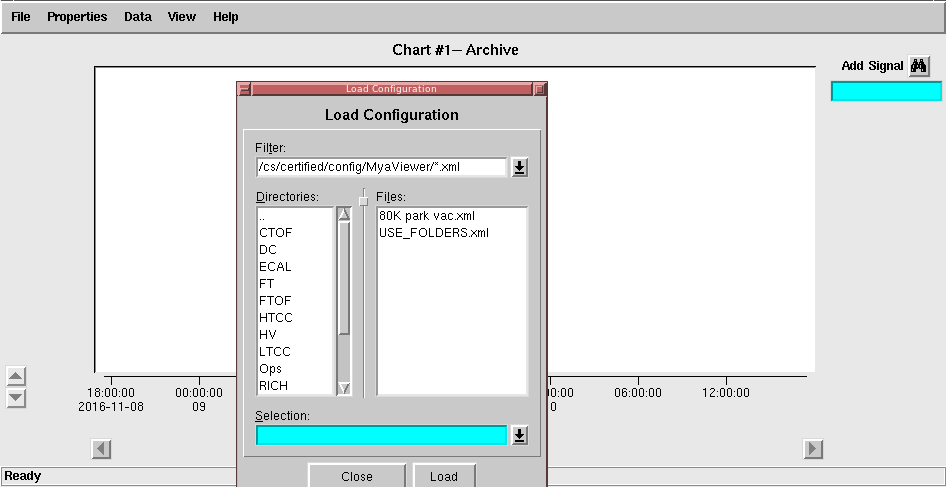
\includegraphics[width=0.7\textwidth]{pics/myaviewer}
    \caption{Utilities for plotting time histories of slow controls variables are accessible from the {\em Tools} section of the CLAS12 main menu (left).  An example of running MyaViewer and opening a preset configuration file via the {\em File $\rightarrow$ Load Config} menu is shown on right.\label{fig:strips}}
\end{figure}

\newpage

\section{Accelerator Screens}
The accelerator's screens are accessed from the main CLAS12 menu via the {\em JMenu} button.  This uses the \texttt{hbops} account on \texttt{hlbl00}, a machine owned and maintained by the accelerator group.  If a prompt requests a username, password, or terminal type, just press {\em Enter}.  The location of the button on the CLAS12 menu and the JMenu screen that should appear are shown in Figure~\ref{fig:jmenu}.

\begin{figure}[htbp]\centering
  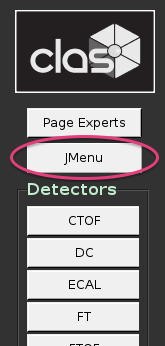
\includegraphics[width=0.16\textwidth]{pics/clas12jmenu}
  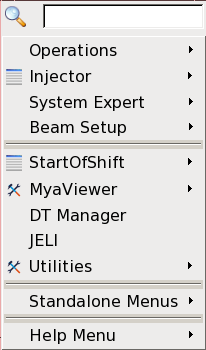
\includegraphics[width=0.2\textwidth]{pics/jmenu}
  \caption{The location of the button to access the accelerator screens from the CLAS12 controls menu (left) and the resulting accelerator JMenu main screen (right).\label{fig:jmenu}}
\end{figure}

\section{Paging System Experts}\label{sec:pagingexperts}
Paging on-call experts is available from the main CLAS12 controls menu via the {\em Page Experts} button at the very top of the screen.  This will open a dropdown menu to choose the desired subsystem, and then open a new window in which to enter a message to be sent to the corresponding expert, as illustrated in Figure~\ref{fig:pageexpert}.
\begin{figure}[htbp]\centering
  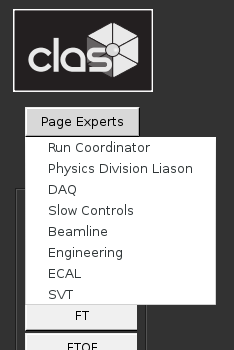
\includegraphics[width=0.2\textwidth]{pics/pageexpert}
  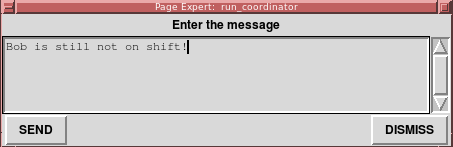
\includegraphics[width=0.6\textwidth]{pics/pageexpertmsg}
  \caption{The dropdown menu for choosing which expert to page (left) and the resulting dialog window in which to enter the message contents (right).\label{fig:pageexpert}}
\end{figure}

\section{Slow Controls Contacts}
The individuals to be contacted for Hall B slow controls are shown in Table \ref{tab:experts}.  The first point of contact for shift operations is always the on-call controls expert, accessible from the paging system described in Section~\ref{sec:pagingexperts} of this document and the phone number in the first row of Table \ref{tab:experts}.  Additional contacts are listed in the table as a fallback.

\begin{table}[htbp]\centering
    \begin{tabular}{llcr}\toprule[1.5pt]
        On-Call & & \ \ \ \ \ 757-748-6922 & \\ \cmidrule[0.5pt]{1-4}
         & Nathan Baltzell & 757-259-5902 & \ \ \ \ \ \texttt{baltzell@jlab.org} \\
         General \ \ \ \ \       & Ken Livingston  &           & \texttt{kliv@jlab.org} \\
                & Wesley Moore & 757-259-6033 &  \texttt{wmoore@jlab.org} \\
                & Bryan McKinnon & & \texttt{mckinnon@jlab.org} \\
        \bottomrule[1.5pt]
    \end{tabular}
    \caption{Hall B slow controls contacts.\label{tab:experts}}
\end{table}

%\bibliography{clas12slow_ops_shift}
\end{document}

